\question \textbf{Local alignment with DP}
  
The DP algorithm can be used to identify optimal local alignments. Assume the scoring scheme as match: 1, mismatch: -1, and gap penalty: 1.

\vspace{0.1 in}

\begin{parts}

%% (a)
  \part Complete the DP table to find the optimal local alignment.

\begin{figure}[h]
      \centering
      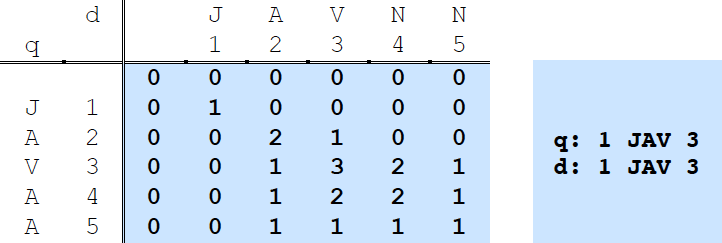
\includegraphics[width=0.7 \textwidth]{fig04/local_dp_solution.png}
\end{figure}

%% (b)
\part Backtrack from $H_{9,6}$ and write down the local alignment.  

\begin{figure}[h]
      \centering
      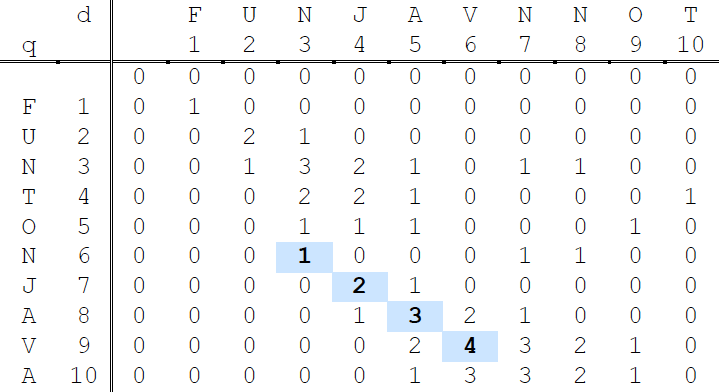
\includegraphics[width=0.75 \textwidth]{fig04/local_dp_backtrack_solution.png}
\end{figure}

\begin{solution}[0.75 in]
\begin{verbatim}
  q: 6 NJAV 9
  d: 3 NJAV 6
\end{verbatim}
\end{solution}

\end{parts}

